\section{Überarbeitung der Sammlungserstellung}\label{sec:uberarbeitung-der-sammlungserstellung}

Das New Collection Modal ist die zentrale Schnittstelle zur Erstellung einer neuen Sammlung auf der Collectiqo-Plattform.
Es ermöglicht Nutzer:innen, grundlegende Eigenschaften wie Presets, Farbauswahl, Name und optional benutzerdefinierte Felder festzulegen.
Im aktuellen Praxismodul wurde das Modal sowohl funktional als auch visuell überarbeitet.

%
\subsection{Frontend}\label{subsec:new-collection-frontend}

Die visuelle und funktionale Überarbeitung des Collection-Modals im aktuellen Praxismodul stellt eine wesentliche Erweiterung gegenüber der vorherigen Version dar.
Abbildung \ref{fig:modal-old} zeigt das ursprüngliche Modal aus dem vorangegangenen Semester.
Hier war es lediglich möglich, eine neue Sammlung durch Auswahl eines vordefinierten Presets zu erstellen.
Benutzerdefinierte Felder konnten nicht ergänzt werden, ebenso fehlte die Möglichkeit, Farben oder Bilder zu hinterlegen.
Für die benutzerdefinierten Felder sowie die Farbauswahl existierten zwar bereits die Frontend Buttons, jedoch waren diese nicht funktional bzw. das Backend konnte mit der Auswahl noch nicht umgehen.

\begin{figure}[H]
    \centering
    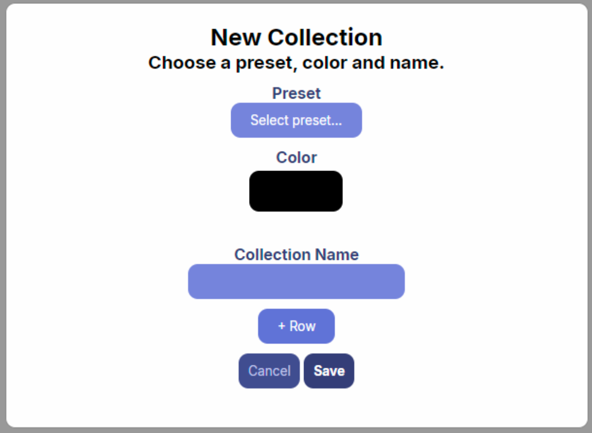
\includegraphics[width=0.6\textwidth]{modal_old}
    \caption{Ursprüngliches Collection-Modal (Praxismodul II)}
    \label{fig:modal-old}
\end{figure}

Die überarbeitete Version, dargestellt in Abbildung~\ref{fig:modal-new}, erweitert diesen Funktionsumfang deutlich.
Neben einer visuell zentrierten und optisch konsistenten Gestaltung wurden mehrere neue Eingabemöglichkeiten ergänzt: Nutzer können nun eigene Felder definieren sowie ein Bild hochladen.
Diese Funktionen korrespondieren direkt mit der im Abschnitt \ref{subsubsec:save-new-collection} beschriebenen Speicherung im Backend.

\begin{figure}[H]
    \centering
    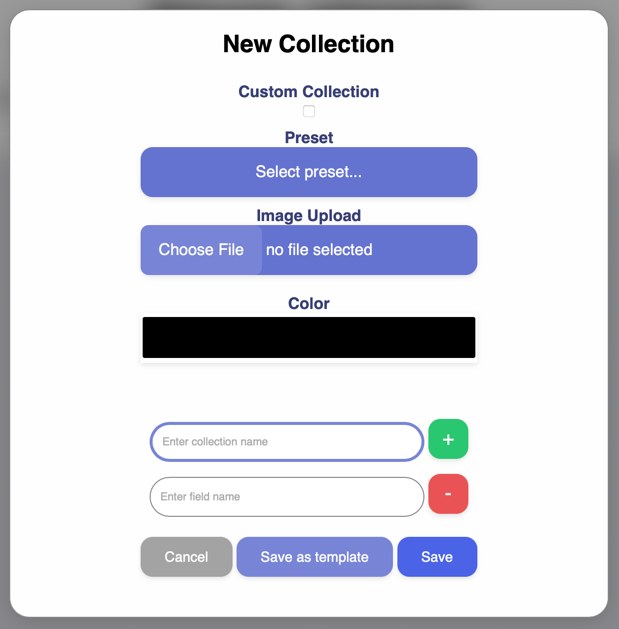
\includegraphics[width=0.6\textwidth]{modal_new}
    \caption{Überarbeitetes Collection-Modal (Praxismodul III)}
    \label{fig:modal-new}
\end{figure}

Zusätzlich zu diesen Eingabefeldern wurden zwei Schaltflächen implementiert: „Save“ und „Save as template“.
Über „Save“ wird die Sammlung wie in Abschnitt \ref{subsubsec:save-new-collection} beschrieben direkt gespeichert, während „Save as template“ eine Vorlage erstellt, die beim nächsten Öffnen des Modals im Preset-Menü ausgewählt werden kann (siehe Abschnitt \ref{subsubsec:save-as-template}).
Beim Wechsel eines Presets wird das Modal dynamisch mit den entsprechenden Daten befüllt – diese Funktionalität ist ebenfalls im Backend dokumentiert (vgl. Abschnitt \ref{subsubsec:load-template-data}).

\subsection{Backend}\label{subsec:new-collection-backend}

Parallel zur Überarbeitung des Frontends wurde auch das Backend des New Collection Modals grundlegend erweitert.
Während im vorherigen Semester lediglich das Erstellen einer Sammlung anhand vordefinierter Presets möglich war, unterstützt das System nun eine deutlich flexiblere und funktionsreichere Erstellung.

\subsubsection{Speichern einer individuellen Sammlung}\label{subsubsec:save-new-collection}

Beim Klick auf den „Save“-Button werden alle eingegebenen Daten – der Sammlungsname, die benutzerdefinierten Spaltennamen, ein Bild sowie eine gewählte Farbe – über ein \texttt{FormData}-Objekt an den Endpunkt \texttt{/create-new-collection} gesendet:

\begin{lstlisting}[language=JavaScript, caption=Clientseitiges Speichern einer neuen Sammlung]
const formData = new FormData();
formData.append('name', collectionName);
formData.append('columns', JSON.stringify(columns));
formData.append('color', color);
formData.append('imageUpload', file);

const response = await fetch('/create-new-collection', {
    method: 'POST',
    body: formData
});
\end{lstlisting}

Der Server verarbeitet diese Daten und speichert die Inhalte in der Datenbank.
Das Bild wird in der MongoDB als Binärdaten abgelegt, die Farbe als Textwert gespeichert.
Die so gespeicherte Sammlung erscheint anschließend in der Übersicht.
Leider wird im Frontend die Auswahl der Farbe und des Bilds nicht weiter verwertet.

Der API-Endpunkt \texttt{/create-new-collection} wird durch den \texttt{createNewCollectionController} verarbeitet, der intern den \texttt{createNewCollectionService} aufruft.
Dieser wurde im aktuellen Praxismodul dahingehend erweitert, dass neben dem Namen, den Spalten und dem Benutzername nun auch ein Bild (als Binärdaten) sowie ein Farbwähler-Wert verarbeitet und in der Datenbank gespeichert werden können.

\begin{lstlisting}[language=JavaScript, caption=Service-Aufruf im Controller]
await createNewCollectionService(
    name,
    parsedColumns,
    username,
    imageBuffer,
    imageType,
    color
);
\end{lstlisting}

Die Speicherung erfolgt in der MongoDB-Collection \texttt{collections} über folgenden Datenbankeintrag:

\begin{lstlisting}[language=JavaScript, caption=Dokumentstruktur im Service]
const doc = {
    name: name,
    columns: columns,
    username: username,
    entries: [],
    color: color,
    image: imageBuffer,
    imageType: imageType
};

const result = await collection.insertOne(doc);
\end{lstlisting}

\subsubsection{Speichern einer Sammlung als Template}\label{subsubsec:save-as-template}

Alternativ zum direkten Speichern kann eine Sammlung auch als Vorlage hinterlegt werden.
Dies geschieht über den „Save as template“-Button, der die Daten an den Endpunkt \texttt{/create-template} sendet:

\begin{lstlisting}[language=JavaScript, caption=Clientseitiges Speichern einer Sammlung als Vorlage]
const formData = new FormData();
formData.append('name', templateName);
formData.append('columns', JSON.stringify(columns));
formData.append('color', color);

const file = document.getElementById('imageUpload').files[0];
if (file) {
    formData.append('imageUpload', file);
}

await fetch('/create-template', {
    method: 'POST',
    body: formData
});
\end{lstlisting}

Der API-Endpunkt \texttt{/create-template} wird durch den \texttt{createTemplateController} verarbeitet.
Dieser ruft intern den \texttt{createTemplateService} auf und übergibt die extrahierten Daten des Formulars, einschließlich der optionalen Bild- und Farbangaben:

\begin{lstlisting}[language=JavaScript, caption=Service-Aufruf im Controller]
await createTemplateService({
    ...templateData,
    image: templateData.imageBuffer,
    imageType: templateData.imageType
});
\end{lstlisting}

Im Service erfolgt die Speicherung des Templates in der Collection \texttt{templates} der Datenbank \texttt{clq\_collections}.
Die Methode wurde im aktuellen Praxismodul erweitert, um Bilddaten als Buffer sowie den MIME-Type zu verarbeiten und dauerhaft zu speichern:

\begin{lstlisting}[language=JavaScript, caption=Speicherung im createTemplateService]
const templatesCollection = db.collection('templates');

await templatesCollection.insertOne({
    ...templateData,
    image: templateData.imageBuffer,
    imageType: templateData.imageType
});
\end{lstlisting}

Durch diese Erweiterung ist es nun möglich, Vorlagen nicht nur mit strukturellen Informationen (z.B. Spaltennamen), sondern auch mit visuellen Eigenschaften wie Farbe und Bild zu versehen.
Diese Templates stehen beim nächsten Öffnen des Modals im Preset-Auswahlfeld zur Verfügung.
Das System lädt die verfügbaren Templates beim Initialisieren des Modals über eine GET-Anfrage:

\begin{lstlisting}[language=JavaScript, caption=Presets beim Laden des Modals laden]
fetch('/get-user-templates')
    .then(response => response.json())
    .then(templateNames => {
        const $presetSelect = document.getElementById('preset');
        $presetSelect.innerHTML = '<option value="x" disabled selected>Select preset...</option>';
        templateNames.forEach(name => {
            const option = document.createElement('option');
            option.value = name;
            option.textContent = name;
            $presetSelect.appendChild(option);
        });
    });
\end{lstlisting}

Der GET-Endpunkt \texttt{/get-user-templates} wird durch einen zugehörigen Controller verarbeitet, der intern den Service \texttt{getUserTemplatesServices(username)} aufruft.
Dieser Service liest alle Vorlagen aus der Collection \texttt{templates}, die entweder dem aktuellen Benutzer oder als global markiert (\texttt{owner: 'GLOBAL'}) gespeichert wurden.

\begin{lstlisting}[language=JavaScript, caption=Service zum Abrufen von Template-Namen]
const db = await connectToDb();
const templatesCollection = db.collection('templates');

const templates = await templatesCollection
    .find({ $or: [ { owner: username }, { owner: 'GLOBAL' } ] })
    .project({ name: 1 })
    .toArray();

return templates.map(template => template.name);
\end{lstlisting}

Dieser Service liefert ein Array von Namen zurück, das anschließend im Frontend in der Preset-Auswahl angezeigt wird.

\subsubsection{Dynamisches Befüllen durch Preset-Auswahl}\label{subsubsec:load-template-data}

Wird eine gespeicherte Vorlage ausgewählt, sendet das Frontend eine Anfrage, um die zugehörigen Felder, die gespeicherte Farbe und ggf. das Bild zu laden.
Anschließend werden die Eingabefelder entsprechend befüllt:

\begin{lstlisting}[language=JavaScript, caption=Preset-Auswahl lädt Felder und Bild]
const response = await fetch(`/get-preset-data?templateName=${selectedPreset}`);
const templateData = await response.json();

clearExistingFields();
populateFieldsFromTemplate(templateData);
setColorPickerValue(templateData.color);
\end{lstlisting}

\textbf{Backend-Logik:} Der GET-Endpunkt \texttt{/get-preset-data} ruft im Hintergrund den \texttt{getPresetDataService(preset)} auf.
Dieser Service wurde erweitert, um ein vollständiges Template-Objekt mit allen gespeicherten Werten zurückzugeben – einschließlich der dynamisch definierten Felder, der ausgewählten Farbe sowie optional des hinterlegten Bilds und dessen MIME-Type.

\begin{lstlisting}[language=JavaScript, caption=Service zum Laden eines Templates]
const getPresetDataService = async(preset) => {
let db;
try {
db = await connectToDb();
const templatesCollection = db.collection('templates');
if (typeof preset !== 'string') {
throw new Error('Invalid preset value');
}
        const template = await templatesCollection.findOne({ name: { $eq: preset } });

        if (template) {
            return template;
        } else {
            console.warn('No template found for preset:', preset);
            return {};
        }
    } catch (error) {
        console.error('Error fetching preset data:', error);
        return {};
    } finally {
        if (db) {
            await closeConnection();
        }
    }
}
\end{lstlisting}

Diese Funktion prüft zunächst die Gültigkeit des übergebenen Werts \texttt{preset}, stellt dann eine Verbindung zur Datenbank her und sucht in der Collection \texttt{templates} nach einem entsprechenden Eintrag.
Wird dieser gefunden, gibt der Service das gesamte Template-Objekt zurück.
Damit können im Frontend alle notwendigen Eingabefelder und Darstellungen korrekt initialisiert werden.

\subsubsection{Unterschied zum vorherigen Semester}\label{subsubsec:comparison-previous}

Im vorherigen Semester war ausschließlich das Erstellen von Sammlungen basierend auf fest programmierten Presets möglich.
Es bestand keine Möglichkeit, benutzerdefinierte Felder zu speichern oder die Sammlung visuell mit Farbe oder Bild anzureichern.
Die neuen Funktionen stellen daher einen erheblichen Fortschritt dar: Sie ermöglichen nicht nur eine flexible Sammlungserstellung, sondern erlauben es auch, Vorlagen für wiederkehrende Strukturen anzulegen und weiterzuverwenden.